\documentclass[a4 paper]{article}
\usepackage[inner=2.0cm,outer=2.0cm,top=2.5cm,bottom=2.5cm]{geometry}
\usepackage{setspace}
\usepackage[ruled]{algorithm2e}
\usepackage[rgb]{xcolor}
\usepackage{verbatim}
\usepackage{subcaption}
\usepackage{amsgen,amsmath,amstext,amsbsy,amsopn,tikz,amssymb}
\usepackage{fancyhdr}
\usepackage[colorlinks=true, urlcolor=blue,  linkcolor=blue, citecolor=blue]{hyperref}
\usepackage[colorinlistoftodos]{todonotes}
\usepackage{rotating}
\usepackage{booktabs}
\usepackage{listings}
\usepackage{xcolor}

%New colors defined below
\definecolor{codegreen}{rgb}{0,0.6,0}
\definecolor{codegray}{rgb}{0.5,0.5,0.5}
\definecolor{codepurple}{rgb}{0.58,0,0.82}
\definecolor{backcolour}{rgb}{0.95,0.95,0.92}

%Code listing style named "mystyle"
\lstdefinestyle{mystyle}{
  backgroundcolor=\color{backcolour}, commentstyle=\color{codegreen},
  keywordstyle=\color{magenta},
  numberstyle=\tiny\color{codegray},
  stringstyle=\color{codepurple},
  basicstyle=\ttfamily\footnotesize,
  breakatwhitespace=false,         
  breaklines=true,                 
  captionpos=b,                    
  keepspaces=true,                 
  numbers=left,                    
  numbersep=5pt,                  
  showspaces=false,                
  showstringspaces=false,
  showtabs=false,                  
  tabsize=2
}

%"mystyle" code listing set
\lstset{style=mystyle}


\newcommand{\ra}[1]{\renewcommand{\arraystretch}{#1}}

\newtheorem{thm}{Theorem}[section]
\newtheorem{prop}[thm]{Proposition}
\newtheorem{lem}[thm]{Lemma}
\newtheorem{cor}[thm]{Corollary}
\newtheorem{defn}[thm]{Definition}
\newtheorem{rem}[thm]{Remark}
\numberwithin{equation}{section}

\newcommand{\homework}[6]{
	\pagestyle{myheadings}
	\thispagestyle{plain}
	\newpage
	\setcounter{page}{1}
	\noindent
	\begin{center}
		\framebox{
			\vbox{\vspace{2mm}
				\hbox to 6.28in { {\bf MATH 118:~Statistics and Probability \hfill {\small (#2)}} }
				\vspace{6mm}
				\hbox to 6.28in { {\Large \hfill #1  \hfill} }
				\vspace{6mm}
				\hbox to 6.28in { {\it Instructor: {\rm #3} \hfill Name: {\rm #5} \hfill Student Id: {\rm #6}} \hfill}
				\hbox to 6.28in { {\it Assistant: #4  \hfill #6}}
				\vspace{2mm}}
		}
	\end{center}
	\markboth{#5 -- #1}{#5 -- #1}
	\vspace*{4mm}
}

\newcommand{\problem}[2]{~\\\fbox{\textbf{Problem #1}}\hfill (#2 points)\newline\newline}
\newcommand{\subproblem}[1]{~\newline\textbf{(#1)}}
\newcommand{\D}{\mathcal{D}}
\newcommand{\Hy}{\mathcal{H}}
\newcommand{\VS}{\textrm{VS}}
\newcommand{\solution}{~\newline\textbf{\textit{(Solution)}} }

\newcommand{\bbF}{\mathbb{F}}
\newcommand{\bbX}{\mathbb{X}}
\newcommand{\bI}{\mathbf{I}}
\newcommand{\bX}{\mathbf{X}}
\newcommand{\bY}{\mathbf{Y}}
\newcommand{\bepsilon}{\boldsymbol{\epsilon}}
\newcommand{\balpha}{\boldsymbol{\alpha}}
\newcommand{\bbeta}{\boldsymbol{\beta}}
\newcommand{\0}{\mathbf{0}}


\begin{document}
	\homework{Homework \#2}{Due: 07/06/21}{Dr. Zafeirakis Zafeirakopoulos}{Gizem S\"ung\"u}{Esra Eryılmaz}{171044046}
	\textbf{Course Policy}: Read all the instructions below carefully before you start working on the assignment, and before you make a submission.
	\begin{itemize}
		\item It is not a group homework. Do not share your answers to anyone in any circumstance. Any cheating means at least -100 for both sides. 
		\item Do not take any information from Internet.
		\item No late homework will be accepted. 
		\item For any questions about the homework, send an email to gizemsungu@gtu.edu.tr.
		\item Submit your homework (both your latex and pdf files in a zip file) into the course page of Moodle.
		\item Save your latex, pdf and zip files as "Name\_Surname\_StudentId".\{tex, pdf, zip\}.
		\item The answer which has only calculations without any formula and any explanation will get zero. 
		\item The deadline of the homework is 07/06/20 23:55.
		\item I strongly suggest you to write your homework on \LaTeX. However, hand-written paper is still accepted \textbf{IFF} your hand writing is \textbf{clear and understandable to read}, and the paper is well-organized. Otherwise, I cannot grade your homework.
		\item You do not need to write your Student Id on the page above. I am checking your ID from the file name.
	\end{itemize}
	
	\problem{1:}{10+10+10+10+10+10+40 = 100}
	\textbf{WARNING:} Please show your OWN work. Any cheating can be easily detected and will not be graded.
	\newline
	\newline
	For the question, please follow the file called manufacturing\_defects.txt while reading the text below.\\
	\newline
	In each year from 2000 to 2019, the number of manufacturing defects in auto manufacturers were counted. The data was collected from 14 different auto manufactory companies. The numbers of defects for the companies are indicated in 14 columns following the year column. Assume that the number of manufacturing defects per auto company per year is a random variable having a Poisson($\lambda$) and that the number of defects in different companies or in different years are independent.\\
	(Note: You should implement a code for your calculations for each following subproblem. You are free to use any programming languages (Python, R, C, C++, Java) and their related library.)\\
	
	\subproblem{a} Give a table how many cases occur for all companies between 2000 and 2019 for each number of defects (\# of Defects).\\
	Hint: When you check the file you will see: \# of Defects = \{0, 1, 2, 3, 4\}.\\
	\newpage
	\begin{table}[htb!]
		\centering
		\begin{tabular}{c|c}
			\begin{tabular}[c]{@{}c@{}}\textbackslash{}\# of\\Defects\end{tabular} & \begin{tabular}[c]{@{}c@{}}\textbackslash{}\# of cases\\in all company \\between the years\end{tabular}  \\ 
			\hline
			0                                                                      &                          144                                                                                \\
			1                                                                      &                           91                                                                               \\
			2                                                                      &                           32                                                                               \\
			3                                                          & 
			11\\
			4                                                                      &                           2                                                                             
		\end{tabular}
		\caption{Actual cases}
		\label{tab1}
	\end{table}
	
	\subproblem{b} Estimate $\lambda$ from the given data. \\
	{\color{purple}\phantom{x}\hspace{6ex}\textit{$\lambda$ = mean = 
	$\frac{events}{time}$ = total number of defects / total number of cases}}\\\\
	{\color{purple}\phantom{x}\hspace{6ex}\textit{Total number of defects = (0 * 144) + (1 * 91) + (2 * 32) + (3 * 11) + (4 * 2) = 196}}\\
	{\color{purple}\phantom{x}\hspace{6ex}\textit{Total number of cases = 144 + 91 + 32 + 11 + 2 = 280}}\\\\
	{\color{purple}\phantom{x}\hspace{6ex}\textit{$\lambda$ = $\frac{196}{280}$ = 0.7}}

	\subproblem{c} Update Table \ref{tab1} in Table \ref{tab2} with Poisson predicted cases with the estimated $\lambda$.\\
	\begin{table}[htb!]
		\centering
		\begin{tabular}{c|c|c}
			\begin{tabular}[c]{@{}c@{}}\textbackslash{}\# of\\Defects\end{tabular} & \begin{tabular}[c]{@{}c@{}}\textbackslash{}\# of cases\\in all companies\\between the years\end{tabular} & \begin{tabular}[c]{@{}c@{}}Predicted \textbackslash{}\# of cases\\in all companies\\between the years\end{tabular}  \\ 
			\hline
			0                                                                      &                           144                                                                               &                139.0439                                                                                                     \\
			1                                                                      &                           91                                                                               &                 97.3307                                                                                                    \\
			2                                                                      &                           32                                                                               &                 34.0658                                                                                                    \\
			3                                                                      &                           11                                                                               &    
			7.9487\\
			4                                                                      &                           2                                                                               &                  1.391                                                                                                
		\end{tabular}
		\caption{Actual vs. Predicted Cases}
		\label{tab2}
	\end{table}
	\subproblem{d} Draw a barplot for the actual cases (Table \ref{tab2} in column 2) and the predicted cases (Table \ref{tab2} column 3) with respect to \# of defecrs. You should put the figure.\\
    \begin{figure}[h!]
      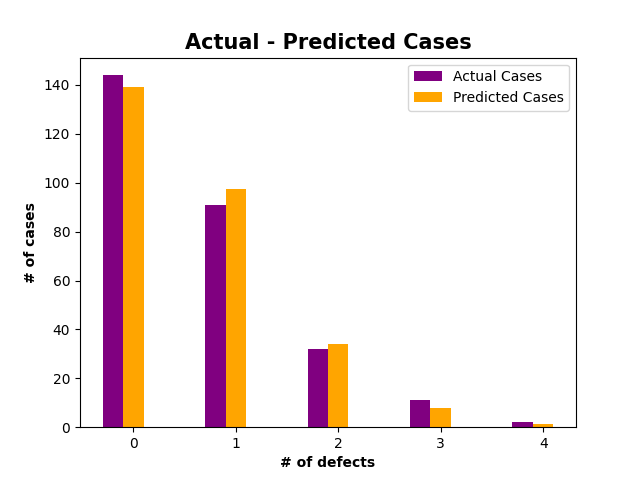
\includegraphics[scale=0.65]{barplot.png}
      \caption{Actual - Predicted Cases}
      \label{fig:barplot}
    \end{figure}
	\newpage
	\subproblem{e} According to the barplot in (c), does the poisson distribution fit the data well? Compare the values of the actual cases and the values of the poisson predicted cases, and write your opinions about performance of the distribution.\\
	{\color{purple}\phantom{x}\textit{As we can see in the barplot, the actual and predicted cases of each defect number are very close to each other.\\}}\\
	{\color{purple}\phantom{x}\hspace{6ex}\textit{Total \# actual cases = 144 + 91 + 32 + 11 + 2 = 280\\}}
	{\color{purple}\phantom{x}\hspace{6ex}\textit{Total \# predicted cases = 139.0439 + 97.3307 + 34.0658 + 7.9487 + 1.391 = 279.7801\\}}\\
	{\color{purple}\phantom{x}\textit{Also total number of actual cases and total number of predicted cases are very close to each other either.\\ So we can say that the poisson distribution fit the data well.\\ Poisson distribution performance is good according to this data.}}\\

	\subproblem{f} According to your estimations above, write your opinions considering your barplot and Table \ref{tab2}. Do you think that road transportation is dangerous for us? Whether yes or no, explain your reason.\\
	{\color{purple}\phantom{x}\textit{(Actual) Total \# defects = (0*144) + (1*91) + (2*32) + (3*11) + (4*2) = 196}}\\
	{\color{purple}\phantom{x}\textit{(Predicted) Total \# defects =(0*139.0439) + (1*97.3307) + (2*34.0658) + (3*7.9487) + (4*1.391) = 194.8724}}\\\\
	{\color{purple}\phantom{x}\hspace{6ex}\textit{While the predicted total number of defects is 194.8724, the actual total number of defects is 196.\\
These numbers are very close to each other, but I think I can still say that road transportation is dangerous for us because the actual number of accidents is higher.}}\\\\


	\subproblem{g} Paste your code that you implemented for the subproblems above. Do not forget to write comments on your code.\\
	Example:\\
	\begin{itemize}
		\item The common code block for all subproblems\\
		Paste here. Your code should read the file and compute other things which the following subproblems need.
		\begin{lstlisting}[language=Python]
import numpy as np
import math
import matplotlib.pyplot as plt

fileName = 'manufacturing_defects.txt'
defects = [0, 1, 2, 3, 4]

# Driver code
def main():
    arr = []
    # Read the file line by line and each line is a list in itself
    with open(fileName, 'r') as infile:
        data = infile.readlines()
        for i in data:
            line = i.split()
            arr.append(line)
    infile.close()

    # Problem a (find total number of cases in all company)
    table1 = number_of_cases(arr)

    # Problem b (find lambda)
    lambdaa, total_case = estimate_lambda(table1)

    # Problem c (find poisson predicted cases with estimated lambda)
    table2 = find_predicted_cases(table1, lambdaa, total_case)

    # Problem d (draw barplot)
    draw_barplot(table2)
        \end{lstlisting}

		\item The code block for (a)\\
		Paste here. Your code should compute the values in Table \ref{tab1} column 2.
		\begin{lstlisting}[language=Python]
# problem a
def number_of_cases(arr):
    table1 = []
    print("\n# of Defects    | # of Cases")
    print("-----------------------------")
    for k in defects:
        count = 0
        for line in arr:
            count = count + line[1:].count(str(k))  # Take each column except first column
        table1.append(count)
        print(k ,"\t\t|\t", table1[k])
    return table1
        \end{lstlisting}

		\item The code block for (b)\\
		Paste here. Your code should compute $\lambda$.
		\begin{lstlisting}[language=Python]
# problem b
def estimate_lambda(table1):
    total_defects, total_case = 0, 0
    for i in defects:
        total_defects += i * table1[i]
        total_case += table1[i]

    lambdaa = total_defects/total_case    # Lambda = total number of defects / total number of cases
    print("\nLambda : " ,lambdaa)
    return lambdaa, total_case
        \end{lstlisting}

		\item The code block for (c)\\
		Paste here. Your code should compute the values in Table \ref{tab2} column 3.
		\begin{lstlisting}[language=Python]
# problem c
def find_predicted_cases(table1, lambdaa, total_case):
    table2 = []
    temp = 0
    print("\n# of Defects    |  # of Cases   |  Predicted # of Cases")
    print("--------------------------------------------------------")

    for k in defects:
        temp = (pow(math.e, -1*lambdaa) * pow(lambdaa, k)) / math.factorial(k)  # apply poisson distribution formula
        temp *= total_case
        temp = round(temp,4)
        table2.append([table1[k], temp])
        print(k ,"\t\t|\t", table2[k][0], "\t|\t" , table2[k][1])

    return table2
        \end{lstlisting}

		\item The code block for (d)\\
		Paste here. Your code should draw the barplot.
		\begin{lstlisting}[language=Python]
# problem d
def draw_barplot(table2):
    # Set width of bar
    barWidth = 0.2

    # Set height of bar
    actual, predicted = [], []
    for i in defects:
        actual.append(table2[i][0])     # height of actual case bar
        predicted.append(table2[i][1])  # height of predicted case bar

    # Set position of bar on X axis
    x_axis = np.arange(len(defects))
    
    # Make the plot
    plt.bar(x_axis, actual, color ='purple', width = barWidth, label ='Actual Cases')
    plt.bar(x_axis + barWidth, predicted, color ='orange', width = barWidth, label ='Predicted Cases')

    plt.title('Actual - Predicted Cases', fontweight ='bold', fontsize = 15)
    plt.xlabel('# of defects', fontweight ='bold', fontsize = 10)
    plt.ylabel('# of cases', fontweight ='bold', fontsize = 10)
    plt.xticks(x_axis + barWidth, defects)

    plt.legend()
    plt.show()
        \end{lstlisting}
	\end{itemize}
	
	
	
	
\end{document} 

